Metode yang akan digunakan dalam penelitian ini adalah \emph{Artificial Neural Network} dengan menggunakan data hasil analisa yang dilakukan oleh Demirbilek pada tahun 2017\cite{DemirbilekReport}. Data tersebut dibagi menjadi 3 bagian, 70 persen data untuk testing, 15 persen data untuk validasi, 15 persen data untuk testing.

Sistem dimulai membaca data langsung dari file dan melakukan pre-processing, data lalu dimasukannya sebagai input ke dalam algoritma ANN untuk melakukan proses training. Konfigurasi model ANN untuk training dibentuk berdasarkan dari hasil optimasi hyperparameter. Setelah training, sistem akan menghasilkan suatu model yang berisi matriks $W$ dan $b (bias)$ di dalamnya.

\subsection{Optimasi Hyperparameter}
\begin{table}[h]
  \caption*{Tabel Batasan Pencarian Hyperparameter}
  \begin{center}
    \begin{tabular}{lrrrr}
      \toprule
      Parameter &        Interval Nilai \\
      \midrule
      Hidden Layer            & {[}1, 5{]}     \\
      Neuron per Layer        & \{3, 5, 8\}    \\
      Prediktor               & \{1, 3\}       \\
      Epoch                   & {[}50, 100, 500, 1000{]} \\
      Model Prediktor         & \{Time Series, Non Time Series\} \\
      LookBack (Time Series)  & {[}1 Detik, 5 Detik, 10 Detik{]}\\
      % Stationary?

      \bottomrule
    \end{tabular}
  \end{center}
  \caption{Tabel batasan pencarian hyperparameter}\label{tab:batasanParameter}
\end{table}

Pembangunan sistem dimulai dengan melakukan optimasi \emph{hyperparameter}. Hyperparameter yang dicari pada proses ini adalah jumlah prediktor, jumlah hidden layer, jumlah neuron, dan jumlah epoch. Karna hyperparameter pada ANN tidak memiliki batasan, maka proses pencarian parameter dibatasi. Batasan-batasan pada parameter, secara lengkap ada pada tabel \ref{tab:batasanParameter}. Metrik yang digunakan untuk melihat performa dari parameter adalah MAPE. 

Tujuan dari proses optimasi hyperparameter adalah untuk mencari model yang optimal dari segi penggunaan memori, waktu komputasi, dan akurasi. Semakin banyak hyperparameter yang digunakan, semakin besar pula memori dan waktu komputasi.

\subsection{Data Set}
Data yang digunakan dalam penelitian ini adalah data dari eksperimen yang di lakukan oleh US Army Corps of Engineer pada Agustus - September 2006. Analisa dilakukan oleh Demirbilek et al dan di tulis dalam laporan yang berjudul \emph{"Laboratory Study of Wind Effect on Runup over Fringing Reefs"}. Data berasal dari hasil percobaan yang dilakukan di Ann Arbor oleh University of Michigan \cite{TechnicalReports}. Data memiliki format \emph{tab separated value (tsv)}, header sensor berlokasi di 
index ke 8 dari baris. Header 1 hingga 7 berisi meta informasi seputar data. Hanya meta informasi frequensi, channels, dan samples yang digunakan untuk TA ini. \emph{Channels} adalah jumlah row yang berisi data, \emph{Samples} adalah jumlah data, dan frequensi adalah jumlah \emph{sample} dari sensor yang diambil dalam waktu 1 detik. Masing-masing berfungsi untuk menentukan proses yang tepat dalam membaca data.
\FloatBarrier
\begin{figure}[h]
  \begin{center}
    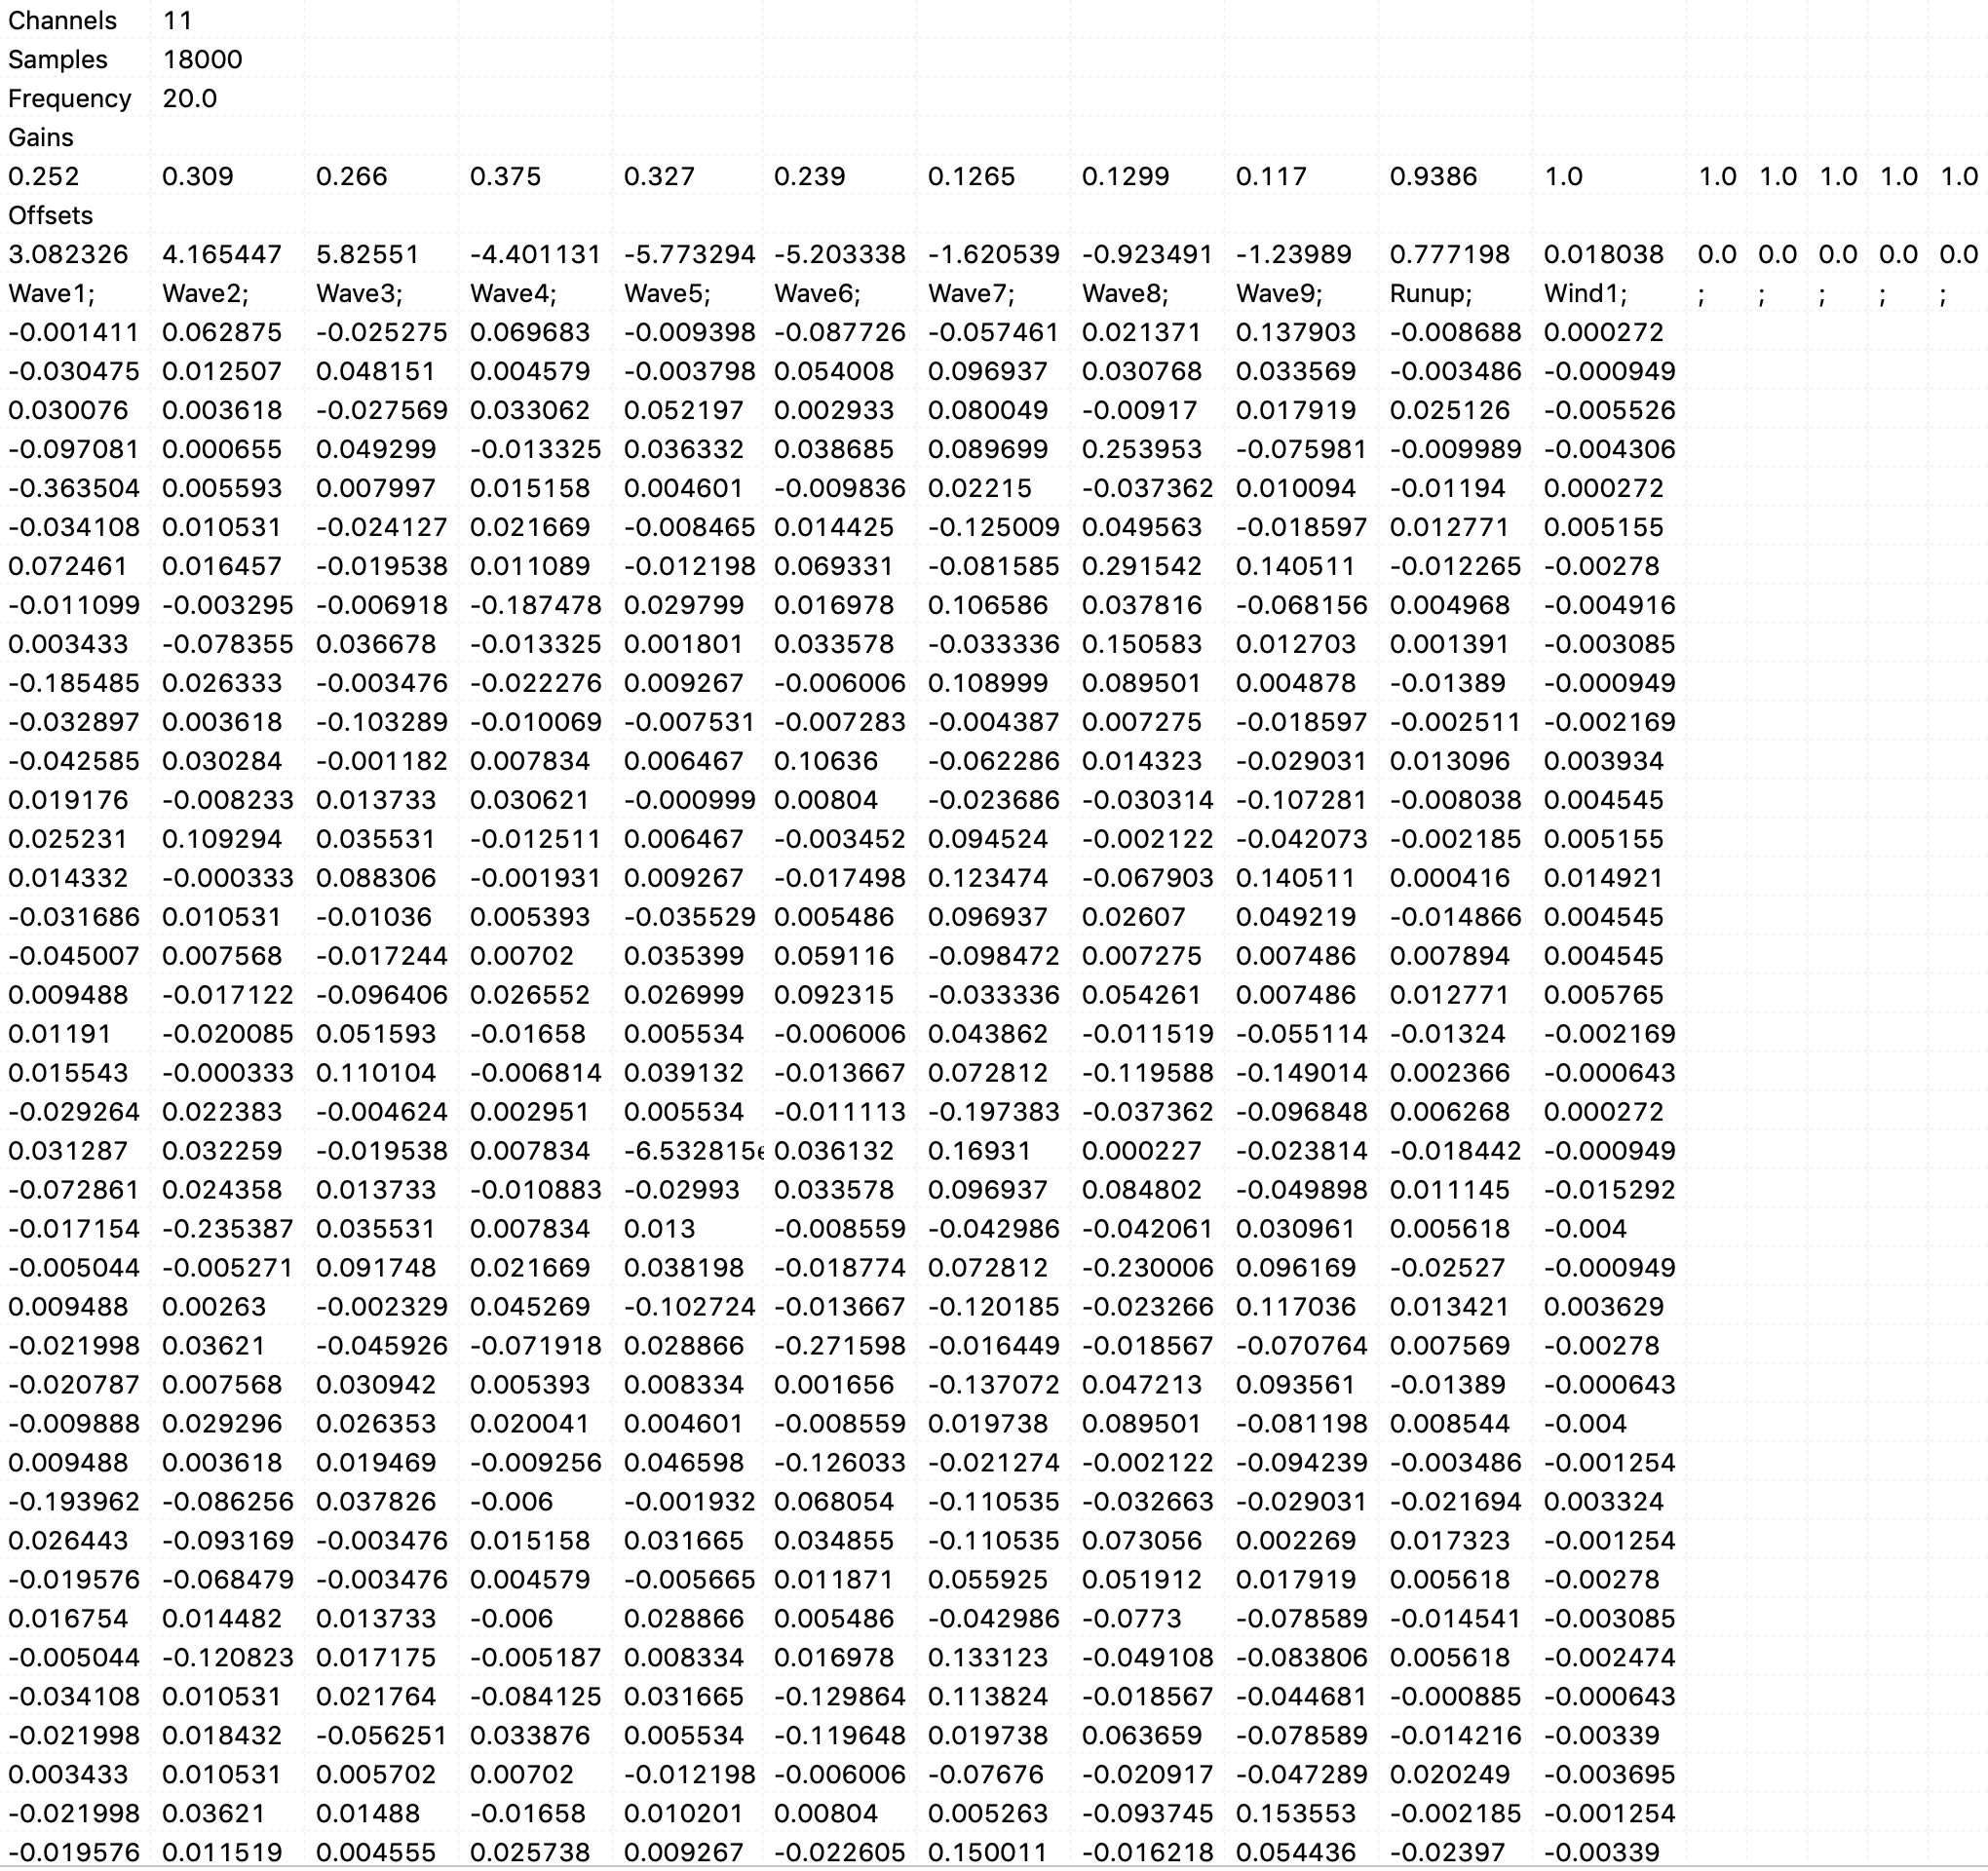
\includegraphics[scale=0.3]{./images/raw_data_test-18.png}
  \end{center}
  \caption{Raw data dengan nama file test-18.dat yang dihasilkan oleh percobaan di laboratorium.}
  \label{fig:raw_data_18}
\end{figure}
\FloatBarrier

\subsection{Kondisi Eksperimen}

\label{kondisiEksperimen}

Eksperimen dibagi menjadi 3 bagian. Eksperimen pertama dilakukan hanya menggunakan variabel gelombang dengan kecepatan angin 0. Eksperimen kedua dilakukan hanya menggunakan variabel angin. Selanjutnya eksperimen ketiga adalah gabungan dari perubahan variable gelombang dan variabel angin.

\begin{figure}[htbp!]
  \begin{center}
    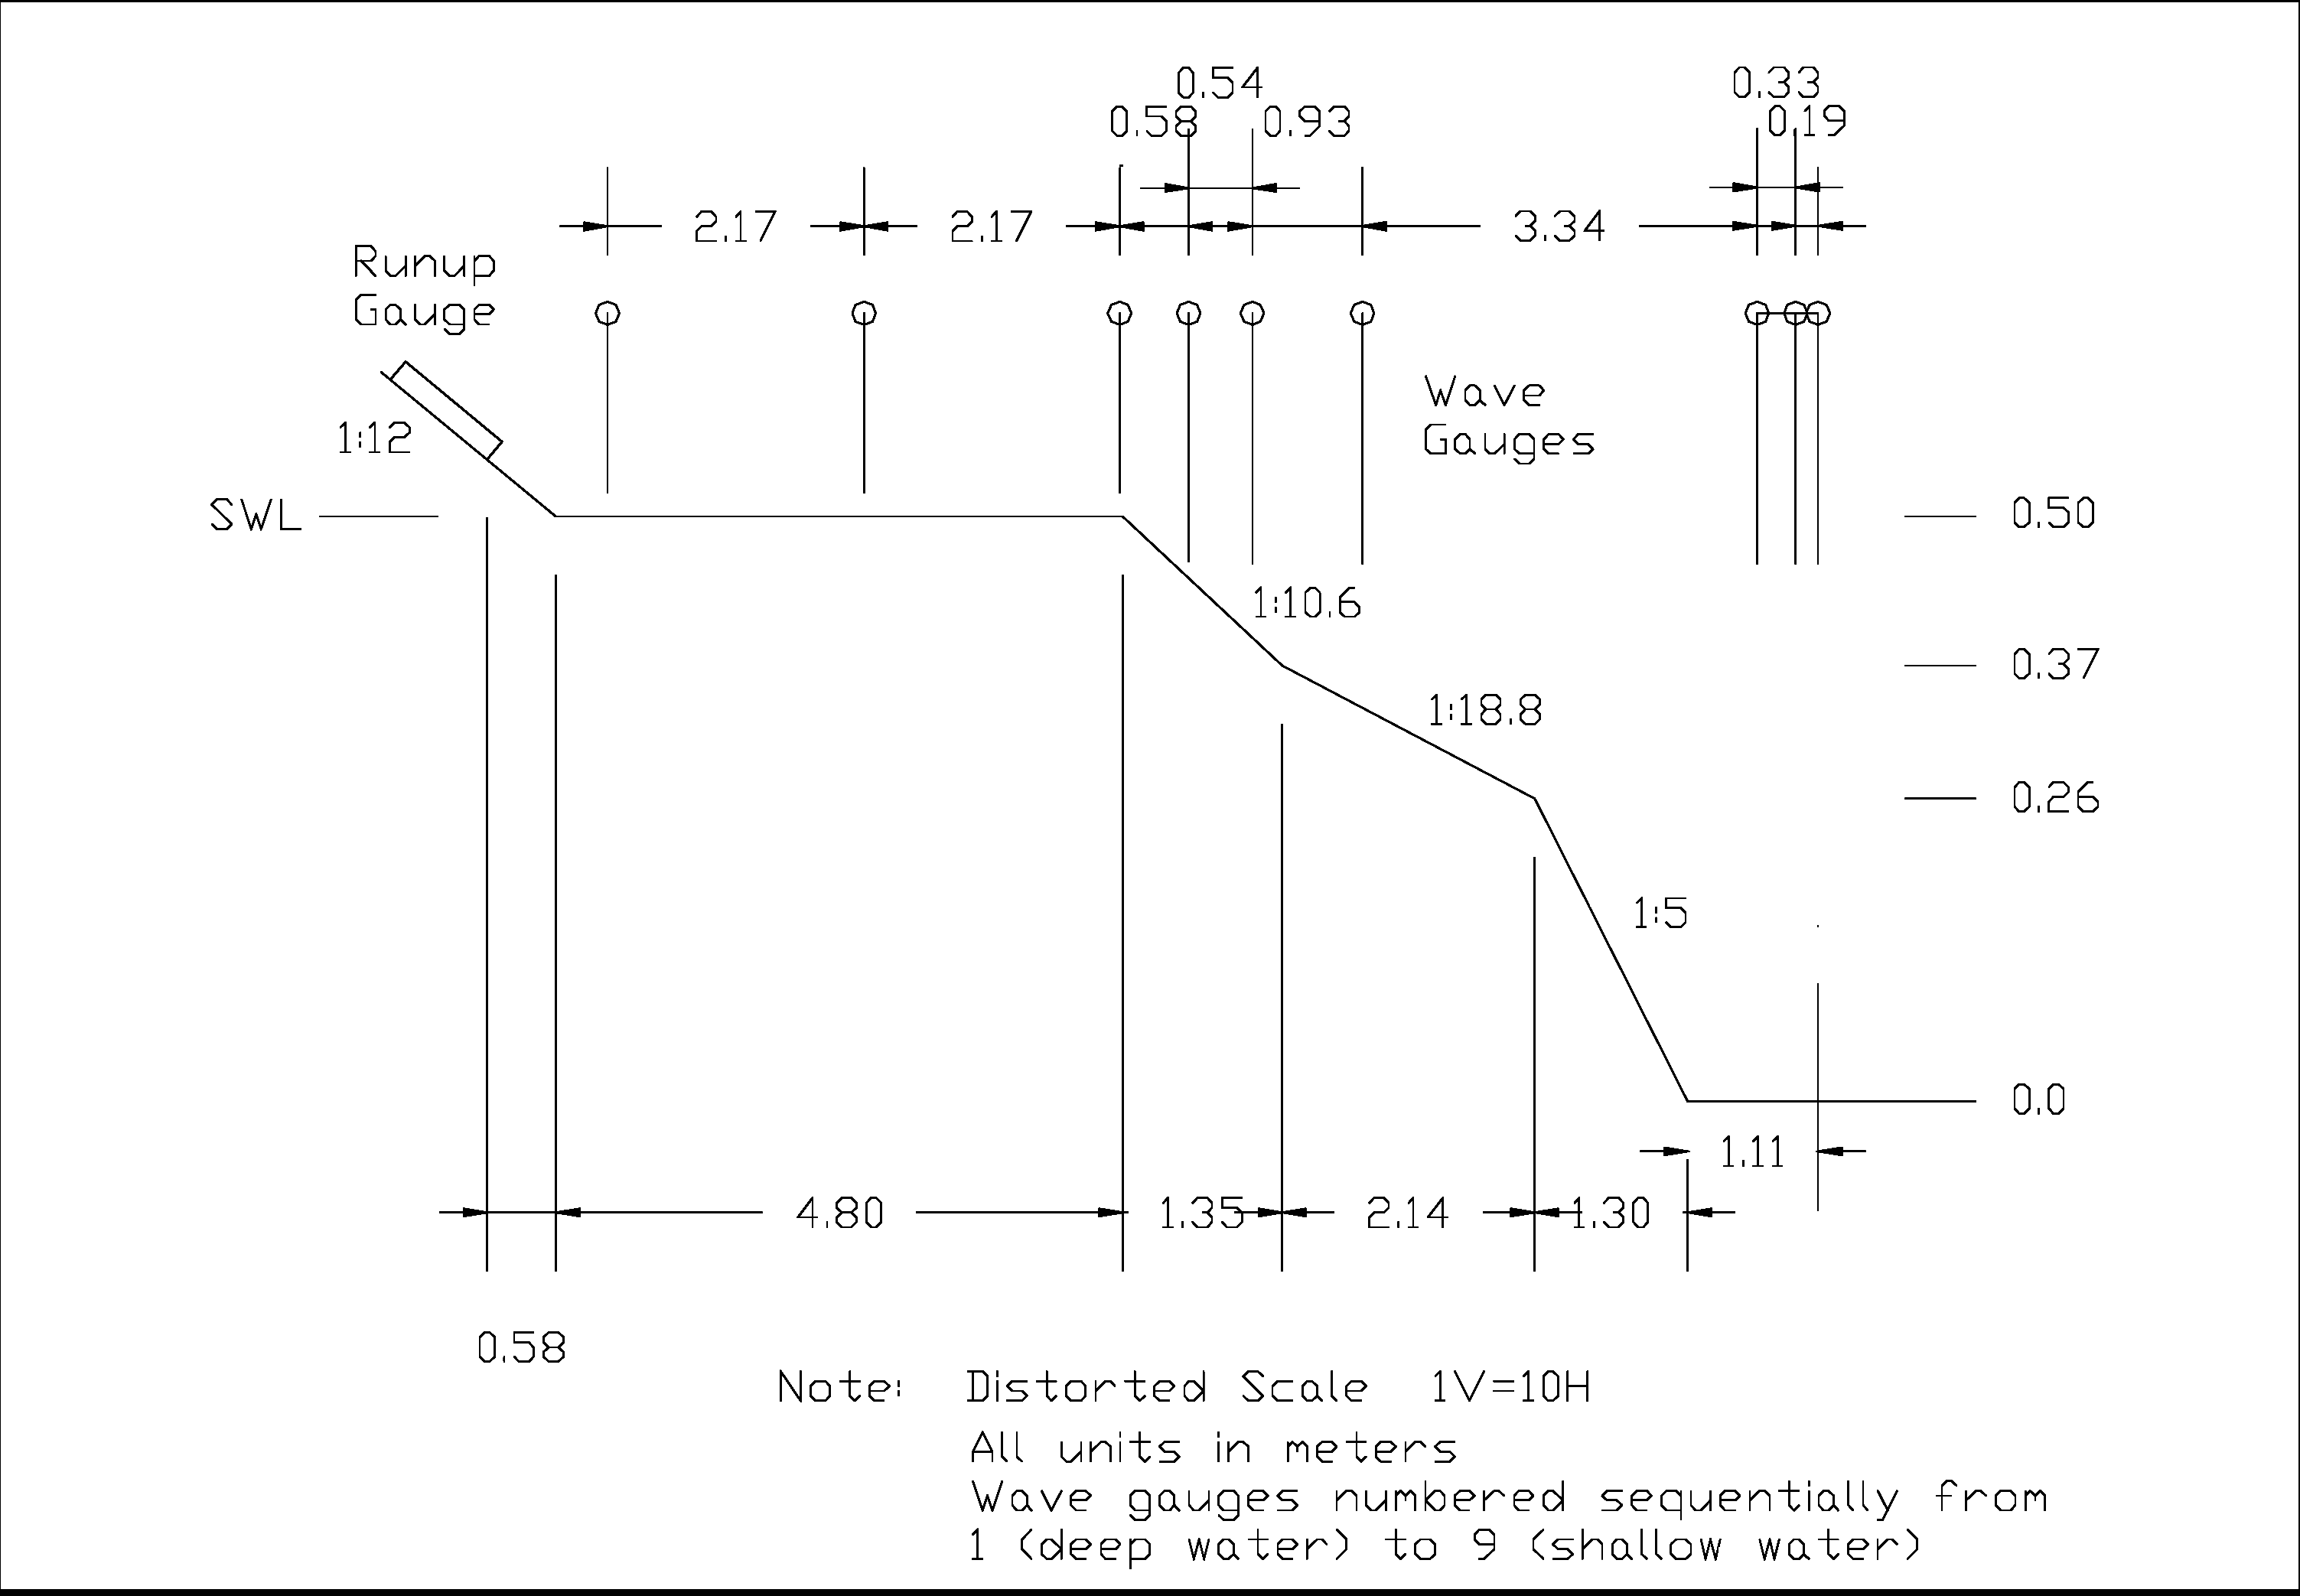
\includegraphics[scale=0.15]{./images/instrumen_eksperimen.png}
  \end{center}
  \caption{Instrumen eksperimen yang digunakan oleh Demirbilek et al \cite{DemirbilekReport}.}
  \label{fig:intrumen_demirbilek}
\end{figure}

Gambar \ref{fig:intrumen_demirbilek} merupakan konfigurasi yang digunakan Demirbilek et al \cite{DemirbilekReport} untuk mengamati gelombang. Pada konfigurasi tersebut ada 9 sensor gelombang, 2 sensor kecepatan angin, dan 1 sensor \emph{runup} gelombang. Wilayah penyebaran sensor gelombang dikelompokan menjadi 2. Wilayah pertama berada di atas karang dan wilayah kedua berada di laut. Wilayah karang merupakan gabungan dari wilayah karang yang datar \emph{Reef Flat} dan wilayah karang yang miring. Wilayah karang datar memiliki panjang mulai dari \emph{SWL} hingga 4.8 meter ke arah laut. Wilayah karang yang miring \emph{Reef Slope} di mulai dari bibir karang datar hingga 4.79 meter ke arah laut. Laut didefinisikan dengan wilayah dengan dasar terdalam. Untuk sensor 1, 2, dan 3 tersebar di wilayah laut, sensor 4, 5, dan 6 tersebar di wilayah \emph{reef slope}, dan untuk sensor 7, 8, dan 9 tersebar di wilayah \emph{reef flat}.

\subsection{Model Artificial Neural Network}
\todo{Ganti model ke timeseries}
Dalam penelitian ini digunakan model ANN dengan 1 output dengan fungsi aktivasi linear (model regresi). Terdapat 3 input, yang berupa vektor dengan masing-masing nilai merupakan sensor 1, sensor 2, dan sensor 3 yang terletak pada laut dalam. Model AAN ini memiliki 1 output dan merupakan model \emph{regressi linear}. Output merupakan prediksi ketinggian \emph{runup} dengan satuan $cm$. Model tersebut direpresentasikan pada gambar \ref{fig:model_ann_ta_ini}.

% \FloatBarrier
\def\layersep{4cm}
\begin{figure}[htp]
  \begin{tikzpicture}[shorten >=1pt,->,draw=black!50, node distance=\layersep]
      \tikzstyle{every pin edge}=[<-,shorten <=1pt]
      \tikzstyle{neuron}=[circle, fill=black!25,minimum size=17pt,inner sep=0pt]
      \tikzstyle{input neuron}=[neuron, fill=green!50];
      \tikzstyle{output neuron}=[neuron, fill=red!50];
      \tikzstyle{hidden neuron}=[neuron, fill=blue!50];
      \tikzstyle{annot} = [text width=4em, text centered]

      % Draw the input layer nodes
      \node[input neuron, pin=left:Sensor 1 t\-1] (I-SENSOR1) at (0,-1) {};
      \node[input neuron, pin=left:Sensor 1 t\-n] (I-SENSOR2) at (0,-2) {};
      \node[input neuron, pin=left:Sensor 3] (I-SENSOR3) at (0,-3) {};

      % Draw the hidden layer nodes
      \path[yshift=0.0cm]{}
          node[hidden neuron] (H-1) at (\layersep,-1 cm) {};
      \path[yshift=0.0cm]{}
          node[hidden neuron] (H-2) at (\layersep,-2 cm) {};
      \path[yshift=0.0cm]{}
          node[hidden neuron] (H-3) at (\layersep,-3 cm) {};
      \path[yshift=0.0cm]{}
          node[hidden neuron] (H-4) at (\layersep,-4 cm) {};

      % Draw the output layer node
      \node[output neuron,pin={[pin edge={->}]right:Prediksi Runup}, right of=H-3] (O) {};

      % Connect every node in the input layer with every node in the
      % hidden layer.
      \foreach \source in {SENSOR1, SENSOR2, SENSOR3}
          \foreach \dest in {1,...,4}
              \path (I-\source) edge node[midway, right] {$W_{hidden}$} (H-\dest);

      % Connect every node in the hidden layer with the output layer
      \foreach \source in {1,...,4}
          \path (H-\source) edge node[midway, right] {$W_{output}$} (O);

      % Annotate the layers
      \node[annot,above of=H-1, node distance=1cm] (hl) {Hidden layer};
      \node[annot,left of=hl] {Input layer};
      \node[annot,right of=hl] {Output layer};
      \label{modelANNTA}
  \end{tikzpicture}
  \caption{Model ANN yang digunakan pada TA ini.}
  \label{fig:model_ann_ta_ini}
\end{figure}
\FloatBarrier


% \subsection{Flowchart Sistem TA}

% Secara keseluruhan, terdapat bentuk hirarki dalam sistem ini. Hirarki \emph{root} (Hirarki Utama), yakni sistem itu sendiri, bertugas sebagai pengatur. \emph{Root} memiliki anak yang memiliki tugas-tugas tertentu, seperti: \emph{Membaca File}, \emph{Transformasi Data}, \emph{Membagi Data}, atau yang paling penting yakni \emph{Training Data}.

\subsection{Flowchart Sistem}

Sistem utama merupakan pengatur dari komponen-komponen yang ada pada sistem TA ini. Komponen-komponen tersebut termasuk: Pembacaan Data, Transformasi Data, Pembagian Data,Inisialisasi Epoch Dan Learning Rate, Melakukan Training, dan Melakukan Testing. Alur kerja lebih lanjut dapat dilihat pada gambar \ref{fig:flowchart_sistem}.

Sistem utama dimulai dengan membaca data. Pembacaan data dibagi menjadi 2. Pembacaan data training dan pembacaan data testing. Data training mencakup 80 persen dari seluruh data observasi, sedangkan data training mencakup 20 persen. Hal ini sejalan dengan Fan et al \cite{fan2008liblinear}, dimana beliau menggunakan rasio 80/20 untuk training dan testing. Setelah melakukan pembacaan data, sistem akan melakukan transformasi data. Mengubah data csv, menjadi matriks dengan panjang kolom \todo{Panjang Kolom}, yang mewakili nilai dari prediktor. Komponen selanjutnya adalah inisialisasi \emph{epoch} dan \emph{learning rate}. \emph{Epoch} adalah representasi dari keseluruhan data yang digunakan pada training. Sedangkan \emph{learning rate} adalah besaran dari suatu langkah pembelajaran. Nilai dari \emph{learning rate} dan \emph{epoch} selanjutnya akan dimasukan ke dalam fungsi training.

\begin{figure}[ht]
  \caption{Flowchart Sistem Utama}
  \begin{center}
    \tikzstyle{decision} = [diamond, draw, 
        text width=4.5em, text badly centered, node distance=3cm, inner sep=0pt]
    \tikzstyle{block} = [rectangle, draw, 
        text width=12em, text centered, minimum height=2em]
    \tikzstyle{circle} = [draw, ellipse, minimum height=2em, distance=4em]
    \tikzstyle{blockTraining} = [rectangle, draw, fill=red!20, 
        text width=12em, text centered, minimum height=2em]
    \tikzstyle{line} = [draw, -latex']
        
    \begin{tikzpicture}[node distance = 1.5cm, auto]
        \footnotesize
        % Place nodes
        \node [circle] (init) {Mulai};
        \node [block, below of=init] (bacaData) {Membaca data report dari csv file};
        \node [block, below of=bacaData] (transformasiData) {Transformasi data menjadi matrix};
        \node [block, below of=transformasiData] (setupEpochLr) {Menentukan jumlah epoch dan learning rate};
        \node [blockTraining, below of=setupEpochLr] (training) {Melakukan Training};
        \node [blockTraining, below of=training] (testing) {Melakukan Testing};
        \node [circle, below of=testing] (stop) {Stop};
      
        % Draw edges
        \path [line] (init) -- (bacaData);
        \path [line] (bacaData) -- (transformasiData);
        \path [line] (transformasiData) -- (setupEpochLr);
        \path [line] (setupEpochLr) -- (training);
        \path [line] (training) -- (testing);
        \path [line] (testing) -- (stop);
        \label{fig:sistem}
    \end{tikzpicture}
  \end{center}
  \label{fig:flowchart_sistem}
\end{figure}
\FloatBarrier

\subsubsection{Flowchart Komponen Training Dan Testing}
\label{FlowChartTraining}

Pada bagian training dan testing \ref{fig:sistem}, algoritma yang digunakan adalah algoritma ANN. Untuk testing, hanya dilakukan algoritma \emph{Feed Forward}. Alur kerja ANN direpresentasikan pada gambar \ref{fig:alur_ann}.

\begin{figure}[ht]
  \caption{Flowchart Komponen Training Dan Testing}
  \begin{center}
    \footnotesize
    \tikzstyle{block} = [rectangle, draw, fill=blue!20, 
        text width=10em, text centered, minimum height=6em]
    \tikzstyle{blockTraining} = [rectangle, draw, fill=red!20, 
        text width=14em, text centered, minimum height=2em]
    \tikzstyle{stopTrainng} = [rectangle, draw, fill=red!20, 
        text width=3em, text centered,  distance=10cm]
    \tikzstyle{line} = [draw, -latex']
    \tikzstyle{circle} = [draw, ellipse, minimum height=2em, distance=4em]
    \tikzstyle{decision} = [diamond, draw, fill=blue!20, 
        text width=4em, text badly centered, node distance=2.5cm, inner sep=0pt]
        
    \begin{tikzpicture}[node distance = 1.5cm, auto]
        % Place nodes
        \node [circle] (init) {Mulai};
        \node [blockTraining, below of=init] (randomWeight) {Inisialisasi $weight$ dengan random data};
        \node [blockTraining, below of=randomWeight] (IW){Mengalikan Input Layer Dengan $Weight$ hidden layer};
        \node [blockTraining, below of=IW] (aktivasi){Jalankan fungsi aktivasi hidden layer};
        \node [blockTraining, below of=aktivasi] (HW){Mengalikan Input Layer Dengan $Weight$ untuk $output$};
        \node [blockTraining, below of=HW] (aktivasiOutput){Menjalankan fungsi aktivasi untuk output neuron};
        \node [blockTraining, below of=aktivasiOutput] (cost){Kalkulasi Error};
        \node [circle, below of=cost] (stop){Stop};
  
        % Draw edges
        \path [line] (init) -- (randomWeight);
        \path [line] (randomWeight) -- (IW);
        \path [line] (IW) -- (aktivasi);
        \path [line] (aktivasi) -- (HW);
        \path [line] (HW) -- (aktivasiOutput);
        \path [line] (aktivasiOutput) -- (cost);
        \path [line] (cost) -- (stop);
    \end{tikzpicture}
  \end{center}
  \label{fig:alur_ann}
\end{figure}
\FloatBarrier

Pada gambar \ref{fig:alur_ann}, algoritma ANN dimulai dengan inisialisasi weight dengan random data(data acak). Selanjutnya, nilai pada \emph{input layer} akan dikalikan dengan $weight$ \emph{hidden layer}, sehingga dihasilkan $a^1$. Untuk menjadi nilai pada \emph{neuron hidden layer} $z^1$, $a$ akan diaktifasi dengan fungsi aktivasi $RELU$ sehingga nilai $z^1$ merupakan hasil dari $relu(a)$. Untuk mengahasilkan nilai prediksi, $z^1$ dikalikan dengan $weight$ pada \emph{output} $W^2$, sehingga mengasilkan $a^2$. Nilai $a^2$ merupakan nilai hasil prediksi, karna fungsi aktivasi dari \emph{output} adalah linear ($f(a) = a$). Lihat gambar \ref{fig:model_ann_ta_ini} untuk representasi dari Model ANN yang digunakan pada TA ini.

\FloatBarrier
